\chapter{servlet}
servlet是运行在web容器中的java程序,很适合用来进行处理web应用中的业务逻辑。

通过servlet和jsp的配合使用,可以使其各负其责:
\begin{itemize}
\item jsp

负责显示页面
\item servlet

负责处理业务逻辑
\end{itemize}
jsp和servlet的使用场景就是:jsp负责页面显示、与用户交互,jsp页面中一些需要处理的数据就送到servlet来处理。
\section{servlet}
通过编写一个负责处理注册信息的servlet来展示servlet的使用方法。

在eclipse中,右键当前的项目,选择新建,找到servlet,即可建立一个servlet(这是一个java类)。

建立完成后,打开刚才建立的servlet,可以看到其中会有一些eclipse自动填写的代码,我们关注的是其中的两个方法doGet和doPost。
一般来说,servlet是用来处理jsp页面传递过来的数据,而传递数据的方式通常情况下是通过表单来进行的,表单中的数据提交通常使用的是post方法。
本部分涉及到两个文件:teacher.jsp和Reg.java,其中teacher.jsp负责页面的显示以及数据的收集,Reg.java负责处理teacher.jsp页面传递过来的数据。
\subsection{jsp页面}
teacher.jsp页面中的关键代码如列表\ref{teacherjsp}所示。
\begin{figure}
\begin{lstlisting}
<form action="teacher_add.jsp" method="post">
<table>
<tr>
  <td>姓名:</td>
  <td><input type="text" name="nm"></td>
</tr>
<tr>
  <td>职工号:</td>
  <td><input type="number" name="staffid" min=20060001 ></td>
</tr>
<tr>
  <td><input type="submit"></td>
  <td><input type="reset"></td>
</tr>
</table>
</form>
\end{lstlisting}
\caption{teacher.jsp中的关键代码}
\label{teacherjsp}
\end{figure}
从列表\ref{teacherjsp}中可以看出,当前form的action是指向的teacher\_add.jsp页面,这是在学习sevlet之前的数据处理方式,从现在开始需要把action的值改为新建的servlet,即:\textcolor{red}{action="Reg"}。
\subsection{servlet代码}
因为teacher.jsp页面中form的数据提交方式为post,所以我们要完成Reg.java中的doPost()方法。Reg.java中的关键代码如列表\ref{reg}所示。
\begin{figure}
\begin{lstlisting}
protected void doPost(HttpServletRequest request, HttpServletResponse response) 
throws ServletException, IOException {
	// 设置request传递过来值的编码,并获取传递值
	request.setCharacterEncoding("utf-8");
	
	String id = request.getParameter("staffid");
	String name = request.getParameter("nm");
	
	//get current date and time
	LabDate ld = new LabDate();
	String time = ld.getDtTm();
	
	//write to database
	String[] fields= {"id","name","logDate"};
	String[] values= new String[3];
	values[0]=id;
	values[1]=name;
	values[2]=time;
	Db db = new Db();
	int i = db.writeDb("teachers", fields, values);
	db.getClose();
	String rz="";
	if(i==1) {
		rz = "done! Will return to the former page in 3 seconds.";
	}else {
		rz = "Something wrong! Will return in 3 seconds.";
	}
	response.getWriter().print(rz);
	//response.setHeader("refresh","3,URL=teacher.jsp");
}
\end{lstlisting}
\caption{Reg.java中的关键代码}
\label{reg}
\end{figure}

\section{filter}
filter是servlet规范中定义的一种特殊类。
filter可以理解成介于客房端和目标资源之间的一个过滤器,即它会对客户端的请示进行过滤后才可以到达服务器上的目标资源,或者访问到目标资源后,对服务器端产生的响应进行处理后才送回客户端(这两个活动可以在一个过滤器中同时进行,即双向过滤)。
filter的示意图如Figure \ref{filter}所示。
\begin{figure}
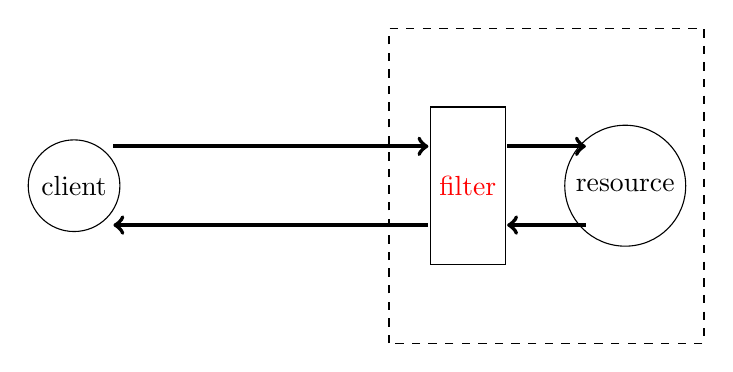
\begin{tikzpicture}
\node (c) at (1,5) [circle,draw] {client};

\node (f) at (6,5) [rectangle,draw,minimum height=20mm] {\textcolor{red}{filter}};
\node (s) at (8,5) [circle,draw] {resource};
\draw [dashed,label=above:webserver] (5,3) rectangle (9,7) ;
\draw [->,line width=1.5pt] (1.5,5.5) -- (5.5,5.5); 
\draw [<-,line width=1.5pt] (1.5,4.5) -- (5.5,4.5); 
\draw [->,line width=1.5pt] (6.5,5.5) -- (7.5,5.5); 
\draw [<-,line width=1.5pt] (6.5,4.5) -- (7.5,4.5); 

\end{tikzpicture}
\caption{the position and function of a filter}
\label{filter}
\end{figure}
在用户注册的时候,如果想禁止某个姓名被使用,可以通过部署一个filter介于注册页面和业务逻辑处理模块之间。接下来的例子中,注册页面为teacher.jsp,业务逻辑处理模块为Reg.java(\textcolor{red}{请注意这是一个servlet})。

\subsection{建立filter}
与建立一个servlet的方法类似,可以建立一个filter,将其命名为FilterReg.java。可以看到这个新建的java文件中,有若干个方法,其中的doFilter方法是我们需要关注的,因为过滤功能就是在此处实现的。Filter文件FilterReg.java的代码如Figure \ref{filterReg}所示。Figure \ref{filterReg}中的代码会判断用户提交的姓名,如果姓名为“zq”,则会截断请求,使得用户请求不能到达Reg这个servlet,从而不能完成注册,达到了禁止特定用户名注册的目的。
\begin{figure}
\begin{lstlisting}
public void doFilter(ServletRequest request, 
 ServletResponse response, FilterChain chain)
 throws IOException, ServletException {
	// TODO Auto-generated method stub
	// place your code here
	HttpServletRequest req = (HttpServletRequest) request; 
	HttpServletResponse resp = (HttpServletResponse) response;
	String id = request.getParameter("staffid");
	String name = request.getParameter("nm");
	//System.out.println("staffid is: "+id);
	System.out.println("filter says: the name is "+name);
	if(name.equals("zq")) {
	  resp.getWriter().println("The name "+name+" is forbidden!");
	}else {
	// pass the request along the filter chain
	  chain.doFilter(request, response);
	  resp.setHeader("refresh", "3,URL=teacher.jsp");
	}
}
\end{lstlisting}
\caption{FilterReg.java中的关键代码}
\label{filterReg}
\end{figure}
\subsection{部署filter}
在上一小节中,讲述了如何建立一个filter,其实要使filter发挥作用还必须进行正确的配置。从servlet 3.0 开始就不需要在web.xml文件中进行配置了,只需要在servlet和filter的源代码文件中进行声明即可,如Figure \ref{webServlet}和Figure \ref{webFilter}所示 。

特别要注意的是filter和servlet里声明的urlPatterns需要保持一致:filter里的@WebFilter(filterName = "/FilterReg",\textcolor{red}{urlPatterns = {"/Reg"}})和servlet里的@WebServlet(name="reg",\textcolor{red}{urlPatterns= {"/Reg"}})。
\begin{figure}
\begin{lstlisting}
package cs;

import java.io.IOException;
import javax.servlet.ServletException;
import javax.servlet.annotation.WebServlet;
import javax.servlet.http.HttpServlet;
import javax.servlet.http.HttpServletRequest;
import javax.servlet.http.HttpServletResponse;

/**
 * Servlet implementation class Reg
 */
@WebServlet(name="reg",urlPatterns= {"/Reg"})
public class Reg extends HttpServlet {
\end{lstlisting}
\caption{servlet中的声明@WebServlet}
\label{webServlet}
\end{figure}
\begin{figure}
\begin{lstlisting}
package filter;

import java.io.IOException;
import javax.servlet.DispatcherType;
import javax.servlet.Filter;
import javax.servlet.FilterChain;
import javax.servlet.FilterConfig;
import javax.servlet.ServletException;
import javax.servlet.ServletRequest;
import javax.servlet.ServletResponse;
import javax.servlet.annotation.WebFilter;
import javax.servlet.http.HttpServletRequest;
import javax.servlet.http.HttpServletResponse;

/**
 * Servlet Filter implementation class FilterReg
 */
@WebFilter(filterName = "/FilterReg",urlPatterns = {"/Reg"})
\end{lstlisting}
\caption{filter中的声明@WebFilter}
\label{webFilter}
\end{figure}

\section{listener}
listener是servlet规范中定义的一种特殊类。listener是监听器,其作用就是用来监听servlet容器中一些事件(event)的发生。从大的分类上来说,listener可以监听以下三个对象的事件:\begin{enumerate}
\item
ServletContex
\item
HttpSession
\item
ServletRequest
\end{enumerate}
listener和event的对应关系,如Table \ref{le}所示。
\begin{table}
\begin{tabular}{ll}
\toprule
\textbf{Listener接口}&\textbf{Event类}\\
\midrule
ServletContextListener&ServletContextEvent\\
ServletContexAttributeListener&ServletContextAttributeEvent\\
HttpSessionListener&\multirow{2}{*}{HttpSeesionEvent}\\
HttpSessionActivationListener&\\
HttpSessionAttributeListener&\multirow{2}{*}{HttpSessionBindingEvent}\\
HttpSessionBindingListener&\\
ServletRequestListener&ServletRequestEvent\\
ServletRequestAttributeListener&ServletRequestAttributeEvent\\
\bottomrule
\end{tabular}
\caption{Listener接口与Event类}
\label{le}
\end{table}

监听器通常可以被用来统计在线人数。接下来以此为例展示监听器的使用方法。
\subsection{新建listener}
与servlet和filter的新建方式一样,新建一个listener。这里需要注意的是,在下一步选择监听事件的时候,选择HttpSessionEvent里面的lifecycle,如Figure \ref{listener}所示,因为这里统计在线人数是通过统计当前活动的session来计数的。
\begin{figure}
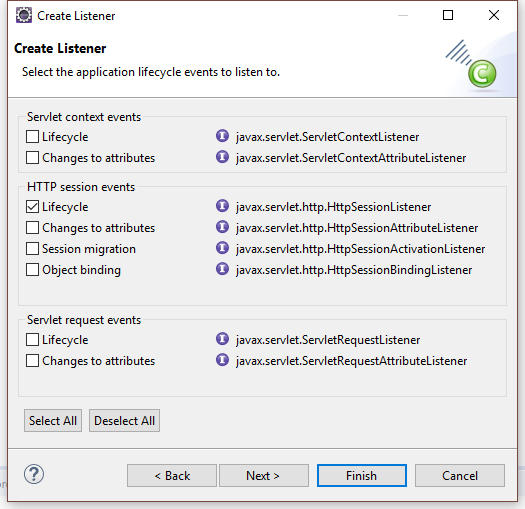
\includegraphics[width=1\linewidth]{servletListener.png}
\caption{选择listener监听事件}
\label{listener}

\end{figure}

其代码如Figure \ref{listenercode}所示。
\begin{figure}
\begin{lstlisting}
package listener;

import javax.servlet.annotation.WebListener;
import javax.servlet.http.HttpSessionEvent;
import javax.servlet.http.HttpSessionListener;

import cs.LabDate;
/**
 * Application Lifecycle Listener implementation class OnlineNum
 *
 */
@WebListener
public class OnlineNum implements HttpSessionListener {
	private int count;
	
	public int getNum() {
		return count;
	}
	
	public synchronized void setCount(int c) {
		count+=c;
	}

    /**
     * Default constructor. 
     */
    public OnlineNum() {
        // TODO Auto-generated constructor stub
    	count=0;
    	System.out.println("当前在线人数被初始化为0");
    }

	/**
     * @see HttpSessionListener#sessionCreated(HttpSessionEvent)
     */
    public void sessionCreated(HttpSessionEvent arg0)  { 
         // TODO Auto-generated method stub
    	String dt = new LabDate().getDtTm();
    	String sid = arg0.getSession().getId();
//    	count++;
    	setCount(1);
    	System.out.println("at "+dt+","+sid+" coming, 当前在线人数为:"+count);
    }

	/**
     * @see HttpSessionListener#sessionDestroyed(HttpSessionEvent)
     */
    public void sessionDestroyed(HttpSessionEvent arg0)  { 
         // TODO Auto-generated method stub
//    	count--;
    	setCount(-1);
    	String dt = new LabDate().getDtTm();
    	String sid = arg0.getSession().getId();
    	System.out.println("at "+dt+","+sid+" leave, 当前在线人数为:"+count);
    }	
}
\end{lstlisting}
\caption{listener代码}
\label{listenercode}
\end{figure}
\subsection{部署listener}
listener的部署很简单,不需要另外配置,在创建listener的时候eclipse会自动帮助创建一条注释:\textcolor{red}{@WebListener},这条注释就完成了listener的部署。

通常,每个http请求都会与一个session关联在一起。如果该请求没有与之相关联的session,那么服务器会为其创建一个session,此时会触发sessionCreated事件;该session会在用户不再活动的一定时间之后失效,或者用户主动注销(调用session.invalidate()方法),此时会触发sessionDestoryed事件,这两个事件会被监听器监听到。

